\section{Java RMI}
Java RMI, short for Java Remote Method Invocation, is a middleware type used with Java, and is used to connect several java machines together.

We will in the following chapter describe how the virtual machine that Java uses to run works, in context to the RMI, and how the RMI works.
\subsection{Java Virtual Machine}
\subsubsection{Java as a programming language}
The semantics of a programming language are designed to be close to the natural language, while it's staying easy for a machine to interpret. Java is a so-called \emph{high-level language} which creates an abstraction from the machine code. High-level code must be interpreted by the machine before it is able to run. Java works with and intermediate language called \emph{Java bytecode} and the \emph{Java Virtual Machine}.

\subsubsection{Java bytecode and JVM}
A Java Virtual Machine (JVM) is a process virtual machine that can execute Java bytecode. It is the code execution component of the Java platform

When a Java project is build, it translates the source code to Java bytecode. This takes the high-level code closer to machine code, and this byte code is a collection of instruction; easier to interpret, but less readable for a machine. Whenever a Java application on a Java enabled platform is running, the Java bytecode is passed to the JVM. The interpreter in the Java Virtual Machine usually starts compiling the entire bytecode at runtime.

The main advantage of this system is the increased compatibility. Since your applications run in a virtual machine instead of directly on your hardware, the developer can program and build their application once, which can then be executed on every device with an implementation of the JVM.

\subsection{RMI architecture layers}
The RMI architecture contains three different layers \footnote{http://publib.boulder.ibm.com/infocenter/javasdk/v5r0/index.jsp?\\topic=\%2Fcom.ibm.java.doc.diagnostics.50\%2Fdiag\%2Funderstanding\%2Frmi\_implementation.html}

\begin{figure}[ht!]
\centering
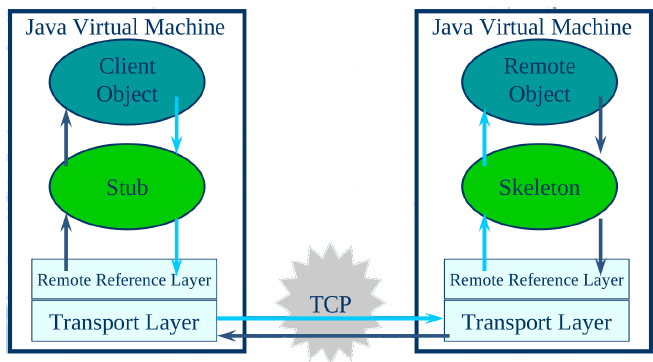
\includegraphics[width=100mm]{img/RMI_layer.png}
\caption{The RMI layers; Stub and skeleton, Remote reference and Transport layer}
\label{Remote Layers}
\end{figure}

\begin{description}
 \item[Stub and skeleton layer] \hfill \\
The stub and skeleton layer, is the "communication" between the client object, and the remote object. This is where the call gets serialized, and again deserialized. This layer holds the reference that the object gets, when calling for a method. The stubs and skeletons are compiler created.

 \item[Remote Reference layer] \hfill \\
This layer manages marshalling and unmarshalling the data, that are handled down from the above layer. It creates a data transmission through a stream oriented connection.

 \item[Transport layer] \hfill \\
Works through a TCP/IP connection, and provides the basic connectivity, such as listening for calls, managing requests, and providing some firewall strategies.
\end{description}

\subsection{Remote interface and remote objects}


A Remote interface is used to create a remote object. An object is remote by implementing the Remote interface. To make it remote, the interface must extend the \emph{java.rmi.Remote} interface. When dealing with a \emph{throws} clause in a method, it must as well declare \emph{java.rmi.RemoteException}, in addition to any other exception.\\

The remote interface and implementation class are then used by RMI to generate a client stub and server skeleton for the remote object. The stub of the object acts as a local representative to the client, and basically is a remote reference.

\begin{figure}[ht!]
\centering
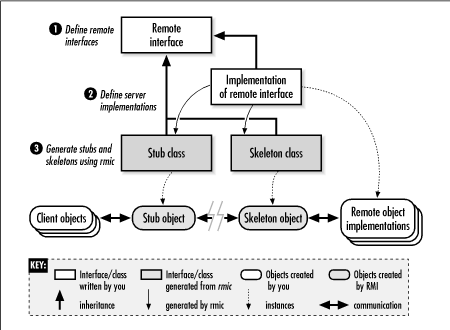
\includegraphics[width=150mm]{img/remote_object_relationship.png}
\caption{ Relationships among remote object, stub, and skeleton classes}
\label{Remote Object relationship}
\end{figure}

\subsection{Remote Method Invocation}
The Java Remote Method Invocation system is a mechanism that enables an object on one Java virtual machine to invoke methods on an object in another Java virtual machine. When such an object is invoked, its arguments are marshalled and sent from the local virtual machine to the remote one, where the arguments are \emph{unmarshalled} and used. When the method terminates, the results are \emph{marshalled} (meaning it must be serializeable) from the remote machine and sent to the caller's virtual machine.

To make a remote object accessible to other virtual machines, a program must register it with the RMI registry.
The program supplies the registry with a string, holding the name of the remote object, and the remote object itself. When a program wants to access the remote object, it only needs to call the registry with name of the object. The registry returns a reference (called stub) of the remote object to the caller. Then, it can invoke methods on the object (through the stub). 